%-------------------------------------------------------------------------------
% SPATIAL DISCRETIZATION 
%-------------------------------------------------------------------------------

\section{Spatial Discretization} \label{sec:spectral}

In order to numerically solve the R4CF problem, we need to approximate the
spatial domain of the continuous problem. This procedure is typically done by
dividing the domain into grid points, forming what is called a mesh. Various
discretization techniques and numerical methods exist for solving partial
differential equations.

The most established ones are finite elements, finite differences, or finite
volume for 3D discretizations. These discretization techniques are referred to
as local techniques because the values and derivatives of a grid point only
affect other nearby points. They employ local basis functions to approximate
the local behavior and offer flexibility in handling irregular and complex
geometries. These techniques are widely adopted in engineering due to their
practical implementation and adaptive refinement capabilities.

Another class of techniques is called spectral methods. These methods act
globally, using basis functions evaluated over the entire domain to approximate
individual grid points. \\

In the following discussion, we will explore why spectral methods are
well-suited for studying the R4CF and its simple 2D geometry. Additionally, the
significance of regularizing the boundary conditions will become clear. Most of
the theory presented in this section is derived from the books \citet{boyd2001}
and \citet{canuto2006}.  It is important to note that this section involves
some simplifications and non rigour to give a broad overview and justify
applying pseudo-spectral Chebyshev discretization for the R4CF problem.

\subsection{Spectral Methods}

Spectral methods encompass a range of global discretization techniques used to
solve differential and integral equations and can be classified into two main
categories. To demonstrate some of the underlying theory for spectral methods,
we will examine a one-dimensional approximation based on a finite series
expansion of $n+1$ points with a basis functions $\psi_i$ and unknown
coefficients $a_i$:

\begin{align}
u(x) \approx u_n(x) = \sum_{i=1}^{n} a_i \, \psi_i. 
\label{eq:approx}
\end{align}

The approximation can be plugged into a differential or integral equation of
the form $Lu=f(x)$ where $L$ is the operator of the equation. To assess the
accuracy of the approximation, we can analyze the residual function, which
gives the error between the approximation and the real solution. We note that
the residual at a point $x$ can depend on all expansion coefficients, hence the
name global. This residual function is formalized within the framework
\emph{the methods of mean weighted residuals}. Spectral and other
discretization methods can be characterized by how they minimize this residual
function. We can distinguish broadly between two categories of spectral
methods. The "interpolating" or "non-interpolating" versions \citep{boyd2001}.
The so-called \emph{pseudo-spectral} or interpolating refers to the strategy of
interpolation points on which the residual function should be exactly zero.
This technique is also referred to as \emph{collocation}. Through the $n+1$
points that are obtained, the coefficients $a_i$ can be determined. The
non-interpolating versions try to use Galerkin's method or Lanczos tau-method
to solve the equation by multiplying with a test-function ($\phi_i$) and by
integrating the equation. This results in the integrated so-called weak form of
the differential equation, and the residual is tried to be satisfied in terms
of the integral. In the case of the widely used Galerkin's method the test
function chosen to be of the form of the approximating (basis) function. In
this sense, the residual is minimized in a weighted manner by multiplying with
the basis function. It can be shown that Galerkin's method gives higher results
than the collocation method. But due to the simplicity of solving the equation
at the collocation point exactly, the pseudo-spectral approach is preferred and
doesn't lose much accuracy. In this study, the spectral method is actually
referring to the pseudo-spectral approach.

From the point of view of interpolation theory using the collocation method is
defacto equivalent to an implicit polynomial interpolation at specified grid
points in the physical space. The question now is how to choose the right
collocation points. It turns out that if we use unevenly spaced grids
corresponding to the roots of orthogonal polynomials (Chebyshev, Fourier or
Lagrange), we get a much better interpolation compared to an evenly spaced
grid. These grids have a Lebesgue constant of order $1$ and, thus, are
conditioning of the interpolation. Further, the Weierstrass approximation
theorem ensures that any bounded function can be approximated as closely as
wanted.

\subsection{Spectral Convergence Rate and Singularities}

A well-condition set of nodes achieve a spectral (exponential) convergence
\citep{meseguer2020} rate. This is different from linear or quadratic
convergence, where the rate is constant and equal to $1$ and $2$. A spectral
convergence rate refers to the fact of having a rate which is potentially
unboundend. To achieve so an unevenly spaced grid, for example obtained by
Chebyshev polynomials are preferred they as they have a small Lebesgue constant
and thus mitigate numerical issues. 

Another point is that singularities in the function to be approximated largely
affect this convergence rate. If the function has singularities, we can't expect
such a convergence rate and due to the global nature of a pseudo-spectral
discretization all the grid points will be affected. Furthermore, the 
gravest singularity dominates the actual convergence rate and domain of
convergence and that singularities outside the domain of interest may effect
the convergence inside the area of interest. 

\subsection{Why Regularizing the four-sided cavity flow?}

Intuitively, it makes sense that the values at the grid point should also go to
infinity at the singularities as the approximated function itself is unbounded.
This can lead to poor approximation quality and render the approximation
useless in those regions due to oscillations \citep{canuto2006}.

This is especially relevant in cases where the problem involves discontinuous
boundary conditions and when the underlying mathematical problem has
singularities, such as vorticity and pressure terms which diverge in the
un-regularized cavity flows.

This limitation is inherent to spectral methods. On the other hand, finite
element methods are less affected by this issue since the singularity only
contributes to a piecewise and low-order polynomial in the vicinity of the
corner.

However, the strength of spectral methods lies in their ability to provide
exact solutions for well-posed boundary conditions, ensuring mathematical
convergence and serving as a benchmark for solvers. In real-world scenarios, as
an example perfect corners rarely exist, and extreme mathematical problems may
not be encountered, mitigating the impact of singularities to some extent.

In the setting of a benchmark solver that uses a pseudo-spectral method to
guarantee a mathematically converged solution, it seems that we have three
essential options now. First, use substraction of the singularity, which was
done by \citep{botella1998}, but this technique is rather complex. Secondly,
one could use rounded borders as the cavity, but this would lead to the fact
that the geometry is not simple anymore, and discretization errors at the corners
are guaranteed. The third option is to make well-posed,
regularized boundary conditions to get an accurate solution to a slightly
different cavity flow problem. In the interest of looking at the original
problem with discontinuous boundary conditions, the regularization should be
almost step-function-like to be similar to the original velocity profile.

\subsection{Pseudo-spectral Discretization}

The preceding sections explored the advantages of employing the pseudo-spectral
approach. However, it has to be stressed that the actual interpolation points
where we do the collocation have yet to be defined. A common choice are the
previously mentioned Chebyshev nodes which are given by the roots of the
Chebyshev polynomial and minimize the approximation error \citep{boyd2001}.
Specifically, the discretization points for Chebyshev can be expressed as:

\begin{align}
x_i = \cos(\frac{i \pi}{n}), \quad j=0, 1,...,n.
\label{eq:cheb_nodes1d}
\end{align}

These definition yields $m+1$ points in the interval $[-1, 1]$. Notably, the
grid points cluster at the boundary. Figure \ref{fig:cheb_grid1d} illustrates a
Chebyshev grid's unevenly spaced grid point distribution.

\begin{figure}[ht]
  \centering

  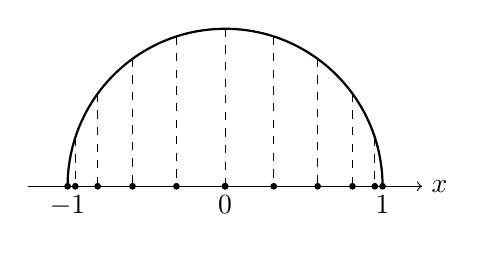
\begin{tikzpicture}
    \def\R{2}
    \def\centerX{0}
    \def\centerY{0}
    
    \draw[thick] (\centerX-\R, \centerY) arc (180:0:\R);
    
    \pgfmathsetmacro{\N}{5}
    
    \foreach \i in {0,...,\N}{
      \pgfmathsetmacro{\angle}{180 - (\i)/(2*\N)*180}
      \pgfmathsetmacro{\x}{\centerX + \R * cos(\angle)}
      \pgfmathsetmacro{\y}{\centerY + \R * sin(\angle)}
      
      \draw[thin, dashed] (\x, \y) -- (\x, \centerY);
      
      \filldraw (\x, \centerY) circle (1pt);
      
      \pgfmathsetmacro{\negx}{\centerX - \R * cos(\angle)}
      \filldraw (\negx, \centerY) circle (1pt);
      \draw[thin, dashed] (\negx, \y) -- (\negx, \centerY);
    }
    
    \node[below] at (\centerX+\R, \centerY) {$1$};
    \node[below] at (\centerX-\R, \centerY) {$-1$};
    \node[below] at (\centerX, \centerY) {$0$};
    
    \draw[->] (\centerX-\R-0.5,\centerY) -- (\centerX+\R+0.5,\centerY) node[right] {$x$};
  \end{tikzpicture}

  \caption{Chebyshev grid visualized as the projection of equally spaced
    points on a unit circle}
  \label{fig:cheb_grid1d}
\end{figure}

Utilizing these points, we can approximate a function within a given 1D domain
and achieve the optimal approximation of Chebyshev polynomials which could be
recovered by going back to the representation with the coefficients $a_i$ (not
discussed here).

\subsection{Chebyshev Differentiation Matrix}

If we would like to approximate derivatives in a discrete setting, using the
concept of differentiation matrices is convenient. A derivate on a given set of
nodes $\{x_0, x_1,..., x_n\}$ with respect to a function $f$, can be written as

\begin{align}
f(x_i)' = f_i' \approx \sum_{j=0}^{n}\mathbf{D}_{ij}f_j.
\end{align}

This formulation is commonly employed for finite difference approximations
where the elements of the differentiation matrix $\mathbf{D}$ correspond to the
derivatives of the respective cardinal functions. In the context of Chebyshev
polynomials, we can utilize the same framework. The Chebyshev grid can be
interpreted as an nth-order finite difference approximation at non-equidistant
grid points. For the 1D Chebyshev nodes, the differentiation matrix is given by
\citep{meseguer2020}:

\begin{align}
\mathbf{D}_{ij} =
\begin{dcases}
  (-1)^{i+j} \frac{\delta_j}{\delta_j(x_i - x_j)},
    & (i \neq j), \\
  \frac{(-1)^{i+j}}{\delta_i} \sum^{n}_{k=0 \, (k \neq i)}
    \frac{\delta_j}{x_i - x_k}, & (i = j).
\end{dcases}
\label{eq:cheb_diff}
\end{align}

As mentioned earlier, the grid points cluster near the boundaries of the
interval, which can result in small differences in function evaluations. The
definition \eqref{eq:cheb_diff} utilizes a numerically more stable formula to
address this issue.

For higher-order derivates, one can calculate them by setting the matrix to the
power of the given order. For instance, s second order is given as follows:

\begin{align}
  f_i'' \approx \sum_{j=0}^{n}\mathbf{D}_{ij}^{2}f_j.
\end{align}

\subsection{2D Chebyshev Discretization}

To define a two-dimensional Chebyshev grid, we can extend the one-dimensional
definition \eqref{eq:cheb_nodes1d} to both spatial directions, $(x_i, y_j)$:

\begin{align} \label{eq:cheb_nodes2d}
  \begin{split}
  x_i & = \cos(\frac{i \pi}{m}), \quad i = 0,1,...,m, \\ 
  y_j &  = \cos(\frac{j \pi}{n}), \quad j = 0,1,...,n
  \end{split}
\end{align}

Figure \ref{fig:cheb_grid2d} shows such a grid. Analogously to the
1D case grid points are clustered in the corner. \\

\begin{figure}[ht]
  \centering
  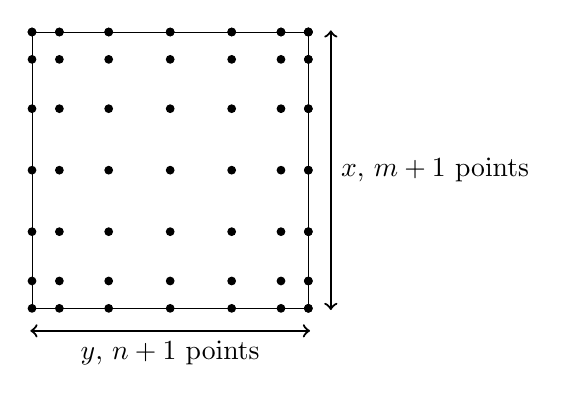
\begin{tikzpicture}[scale=1.2]
  \def\n{7}

  \def\length{3}
  \def\dotsize{0.04}

  \draw (\dotsize,\dotsize) rectangle (\length-\dotsize,\length-\dotsize);

  \foreach \x in {0,...,\n} {
    \foreach \y in {0,...,\n} {
      \pgfmathsetmacro\xx{\length/2*(1-cos((\x+0.5)*180/\n))}
      \pgfmathsetmacro\yy{\length/2*(1-cos((\y+0.5)*180/\n))}
    
      \filldraw[black] (\xx,\yy) circle (\dotsize);
    }
  }

  \draw[<->, thick] (\dotsize/2, -0.2) -- node[below] {$y$, $n+1$ points} (\length-\dotsize/2, -0.2);
  \draw[<->, thick] (\length + 0.2, \dotsize/2) -- node[right] {$x$, $m+1$ points}
    (\length + 0.2, \length - \dotsize/2);
  \end{tikzpicture}
  \caption{2D Chebyshev grid points in a square domain ($m = n$).}
  \label{fig:cheb_grid2d}
\end{figure}

The next step is to define differentiation in the $x$ and $y$ direction of the
grid of a function. One approach is to use the Kronecker delta product
($\mathbf{D} = \mathbf{D_x} \otimes \mathbf{D_y}$) to create the differentiation
matrix for a 2D scalar function $f(x,y)$ \citep{trefethen2000}. Each unknown
value of the function corresponds to an element in a flattened vector. The
differentiation matrices in both spatial directions are combined into a single
large matrix $\mathbf{D} \in \mathbb{R}^{(m+1)(n+1)\times(m+1)(n+1)}$. This
matrix is multiplied by the vector to compute the derivatives. Although the
matrix is not completely dense, higher derivatives result in a dense matrix. \\

Another approach is to consider the grid points in terms of a matrix. Instead
of representing the unknown values as a flattened vector, we can use a matrix
$\Psi \in \mathrm{R}^{(m+1) \times (n+1)}$, where the grid points $ij$
correspond to the $ji$-th entry of the matrix $\Psi$. The spatial derivative of
one grid point is then given by the relations \eqref{eq:discr_der} (Einsteins
summation notation). All derivatives can then simple be obtained the
derivatives by multiplying $\mathbf{D_x}$ from the left with $\Psi$ for the
$x$-derivative and $\Psi \mathbf{D_y}^T$ for the $y$-derivative. The matrix
$\Psi$ is shown in figure \ref{fig:bc_psi}.

\begin{align}
  \begin{split}
  \partial_x \Psi_{ij} = (\mathbf{D_x})_{ik} \Psi_{kj} \\
  \partial_y \Psi_{ij} = (\mathbf{D_y})_{jl} \Psi_{il}
  \end{split}
\label{eq:discr_der}
\end{align}

For the streamfunction equation \eqref{eq:str}, the discrete Laplace operator
$\Delta_{dis} \Psi$ and the biharmonic operator are defined as:

\begin{align}
  \Delta_{dis} \Psi &= \mathbf{D_x}^2\Psi + \Psi{\mathbf{D_y}^2}^T \\
  \Delta_{dis}^2 \Psi &= \mathbf{D_x}^2(\Delta_{dis} \Psi) (\Delta_{dis}
    \Psi){\mathbf{D_y}^2}^T 
\end{align}

Combining all the above, we can state the discrete streamfunction equation we
want to solve numerically:

\begin{align}
\partial_t (\Delta_{dis} \Psi) = \frac{1}{\Rey} \Delta_{dis}^2 \Psi
  + \mathbf{D_x}\Psi((\Delta_{dis}\Psi)\mathbf{D_y}^T)
  - \Psi\mathbf{D_y}^T (\mathbf{D_x}(\Delta_{dis} \Psi)). 
\label{eq:str_dis}
\end{align}

As mentioned, $\Psi$ is a matrix representing the finite-dimensional
approximation of the streamfunction and the matrix $\Delta_{dis} \Psi$ is the
discrete Laplace of $\Psi$. The partial derivative with respect to time will be
discussed in section \ref{sec:time} on temporal discretization.

\subsection{Incorporating the Boundary Conditions} \label{sec:bc}

As seen in the section before, it is convenient for the R4CF to view the grid
points as the transpose of the matrix $\Psi$, and so we can do derivation in
$x$ and $y$ by just applying a matrix multiplication from the left or right
with $\mathbf{D_x}$ or the transpose of $\mathbf{D_y}$ respectively. 

Incorporating the boundary conditions has to be carefully considered and can be
done in many different ways. One possible option is to explicitly substitute
the discrete equations into the equations for the boundary conditions (see
\cite{meseguer2020}). As we will see in our case, the boundary conditions are
simple enough to make the evaluation efficient.

Recalling the tangential boundary conditions \eqref{reg_u_bca},
\eqref{reg_u_bcb} and the definition of the stream function
\eqref{eq:str_defx}, \eqref{eq:str_defy} we see that the boundary conditions
are essential of type Dirichlet as the streamfunction is defined through the
derivative of the two velocity components. For clarity, this is shown below:

\begin{eqnarray}
\frac{\partial\Psi(x,\pm 1,t)}{\partial y} & = & \pm\left[\left(\rme^{k_0(x - 1)} - 1\right)
  \left(\rme^{-k_0(x + 1)} - 1\right)\right]^2,\label{reg_psi_bca} \\
  \frac{\partial\Psi(\pm 1,y,t)}{\partial x} & = & \mp\left[\left(\rme^{k_0(y - 1)} - 1\right)
  \left(\rme^{-k_0(y + 1)} - 1\right)\right]^2.\label{reg_psi_bcb}
\end{eqnarray}

Furthermore, as stated, the boundary components are only nonzero in the
tangential direction of the four lids, meaning this corresponds to the derivate
of the streamfunction normal to the boundary. Regarding the normal component of
the velocity, we can us the fact is that the streamfunction is defined up to a
constant. And the streamfunctions values can be set to $0$ at all the
boundaries (outermost rows and columns of the matrix). As the geometric shape
of the cavity is a square or rectangle, this tells us that the derivative of
the streamfunction along the lids is $0$. Corresponding to the normal component
of the velocity field, which ensures no flux outwards from within the cavity.

We want to now incoorporate the boundary conditions above \eqref{reg_psi_bca}
and \eqref{reg_psi_bcb}, by expressing the first inner grid points (outermost
are all $0$) in terms of the other components. Using the Einstein summation
convention, we can express the derivative of the horizontal walls for the
streamfuncton as,

\begin{align}
\partial_x \Psi_{0j} = \sum_{k=0}^{m} (\mathbf{D_x})_{0k} \Psi_{kj}
  &= \mycancel{=0}{\mathbf{D_x}_{00}\Psi_{kj}} + (\mathbf{D_x})_{01}\Psi_{1j} 
  + (\mathbf{D_x})_{0m-1}\Psi_{m-1j} +  \mycancel{=0}{(\mathbf{D_x})_{0m}\Psi_{mj}}
  + (\mathbf{D_x})_{0\bar{k}}\Psi_{\bar{k}j} \nonumber \\
  &= (\mathbf{D_x})_{01}\Psi_{1j} + (\mathbf{D_x})_{0m-1}\Psi_{m-1j}
  + \mathbf{D_x}_{0\bar{k}}\Psi_{\bar{k}j}, \\
\partial_x \Psi_{nj} = \sum_{k=0}^{m} (\mathbf{D_x})_{mk} \Psi_{kj}
  &= (\mathbf{D_x})_{m1}\Psi_{1j} + (\mathbf{D_x})_{mm-1}\Psi_{m-1j} 
  + (\mathbf{D_x})_{m\bar{k}}\Psi_{\bar{k}j}.
\end{align}

The same is the case for the derivatives in the $y$ direction. $\bar{k}$ is
denoted as the index running from $k=1$ to $k=m-1$.

We can express the above relations as a matrix equation:

\begin{align}
\underbrace{\begin{bmatrix} (\mathbf{D_x})_{01} & (\mathbf{D_x})_{0m-1} \\
    (\mathbf{D_x})_{01} & (\mathbf{D_x})_{0m-1} \\
\end{bmatrix}}_{A \in \mathrm{R}^{2 \times 2}}
\begin{bmatrix} \Psi_{1j} \\ \Psi_{m-1j}
\end{bmatrix} &=
\begin{bmatrix}
\partial_x\Psi_{0j} - (\mathbf{D_x})_{0\bar{k}}\Psi_{\bar{k}j} \\
\partial_x\Psi_{mj} - (\mathbf{D_x})_{m\bar{k}}\Psi_{\bar{k}j} \\
\end{bmatrix}, \nonumber \\
\begin{bmatrix} \Psi_{1j} \\ \Psi_{m-1j}
\end{bmatrix} &=
\underbrace{\begin{bmatrix} a_{11} & a_{12} \\ a_{21} & a_{22} 
\end{bmatrix}}_{A^{-1}}
\begin{bmatrix}
\partial_x\Psi_{1j} - (\mathbf{D_x})_{0\bar{k}}\Psi_{\bar{k}j} \\
\partial_x\Psi_{mj} - (\mathbf{D_x})_{m\bar{k}}\Psi_{\bar{k}j} \\
\end{bmatrix}.
\label{eq:mat1}
\end{align}

The above matrix equation tells us that all elements on the first inner grid
points for the horizontal components are explicitly given through the boundary
conditions. The $2 \times 2$ matrix to the left is known in advance from the
Cheyshev differentiation matrix. It follows that the inverse can be precomputed
and reused in succeeding calculations whenever the boundary conditions have to
be evaluated. The right part of the equations is given through the partial
derivates and a sum of a matrix-vector product of the inner elements $\Psi$.

The same procedure can be done for the $y$ derivatives of the streamfunction at
the vertical wall. Similarly, we get again a matrix that can be pre-stored. 

\begin{align}
\begin{bmatrix} \Psi_{i1} \\ \Psi_{in-1}
\end{bmatrix} &=
\underbrace{\begin{bmatrix} b_{11} & b_{12} \\ b_{21} & b_{22} 
\end{bmatrix}}_{B^{-1}}
\begin{bmatrix}
\partial_y\Psi_{i0} - (\mathbf{D_y})_{0\bar{l}}\Psi_{i\bar{l}} \\
\partial_x\Psi_{in} - (\mathbf{D_y})_{n\bar{l}}\Psi_{j\bar{l}} \\
\end{bmatrix}.
\label{eq:mat2}
\end{align}

One subtlety is that the calculations for the boundary conditions for the
horizontal and vertical walls have to be done one after the other, as the
outermost values in the first rows or columns are dependent. Figure
\ref{fig:bc_psi} shows in blue and red background the two inner rows and
columns which are computed with equation \eqref{eq:mat1} and \eqref{eq:mat2}.

\begin{figure}[ht]
  \centering
  \begin{tikzpicture}

    \matrix (m) [matrix of math nodes, nodes in empty cells,
                 minimum width=1.1cm]
    {
      \Psi_{00} & \Psi_{01} & \dots & \Psi_{0j} & \dots & \Psi_{0n-1} & \Psi_{0n} \\
      \Psi_{10} & \Psi_{11} & \dots & \Psi_{1j} & \dots & \Psi_{1n-1} & \Psi_{1n} \quad \\
      \vdots & \vdots & \ddots & \vdots & \reflectbox{$\ddots$} & \vdots & \vdots \\
      \Psi_{i0} & \Psi_{i1} & \dots & \Psi_{ij} & \dots & \Psi_{in-1} & \Psi_{0n} \\
      \vdots & \vdots & \reflectbox{$\ddots$} & \vdots & \ddots & \vdots & \vdots \\
      \Psi_{m-10} & \Psi_{m-11} \quad & \dots & \Psi_{m-1j} & \dots & \Psi_{m-1n-1} & \Psi_{m-1n} \\
      \Psi_{m0} & \Psi_{m1} & \dots & \Psi_{mj} & \dots & \Psi_{m-1n} & \Psi_{mn} \\
    };

    \begin{scope}[on background layer]
      \fill[red!10] (m-1-1.south) rectangle (m-6-2.north east);
      \fill[red!10] (m-1-7.south) rectangle (m-6-6.north west);
      \fill[blue!10] (m-1-1.north) rectangle (m-2-7.south);
      \fill[blue!10] (m-6-1.south) rectangle (m-6-7.north);
    \end{scope}

    \begin{scope}[on background layer]
      \fill[gray!10] (m-1-1.north west) rectangle (m-1-7.south east);
      \fill[gray!10] (m-7-1.south west) rectangle (m-1-1.north east);
      \fill[gray!10] (m-7-1.south west) rectangle (m-7-7.north east);
      \fill[gray!10] (m-7-7.south west) rectangle (m-1-7.north east);
    \end{scope}

    \draw [decorate,decoration={brace,amplitude=5pt},xshift=-0.5cm,yshift=0.3cm] (m-7-1.south west) -- (m-1-1.north west) node [black,midway,xshift=-0.5cm] {$x$};
    \draw [decorate,decoration={brace,amplitude=5pt},xshift=0.3cm,yshift=0.5cm] (m-1-1.north west) -- (m-1-7.north east) node [black,midway,yshift=0.5cm] {$y$};
  \end{tikzpicture}
  \caption{Elements of streamfunction matrix needed for the boundary calculation}
  \label{fig:bc_psi}
\end{figure}
